\documentclass[ aps, pra, reprint, notitlepage ]{revtex4-1}

\usepackage{graphicx}% Include figure files
\usepackage{dcolumn}% Align table columns on decimal point
\usepackage{bm}% bold math
\usepackage{amsmath}
\usepackage{amssymb}
\usepackage{tabularx}

\begin{document}

%Title of paper
\title{Analysis of Fire Fighting Methods using Cellular Automaton Modeling}

% repeat the \author .. \affiliation  etc. as needed
% \email, \thanks, \homepage, \altaffiliation all apply to the current
% author. Explanatory text should go in the []'s, actual e-mail
% address or url should go in the {}'s for \email and \homepage.
% Please use the appropriate macro foreach each type of information

% \affiliation command applies to all authors since the last
% \affiliation command. The \affiliation command should follow the
% other information
% \affiliation can be followed by \email, \homepage, \thanks as well.

\author{Matthew Wilson}

\author{Brent D. Foy}
\affiliation{Department of Physics, Wright State University, Dayton, OH 45435, USA}

\date{\today}

\begin{abstract}
	% insert abstract here
	
\end{abstract}

%\maketitle must follow title, authors, abstract, \pacs, and \keywords
\maketitle

% body of paper here - Use proper section commands
% References should be done using the \cite, \ref, and \label commands

\section{\label{Intro}Introduction}

\subsection{\label{ForestFires} Forest Fires and their Effects}

In early November of 2018, a forest fire started near Camp Creek Road in Butte County, California, grew until it was finally contained on November 25th. In this time the fire burned over 150,000 acres of land with mass evacuations for nearby towns.\cite{CampFire, CampFireReport} While this was the largest single wildfire in California's history, 2018 was only the 5th largest year of burned acres in the past decade with over 2.2 million acres burned in 2017.\cite{WildFireYear}

%\begin{figure}[ht]
%	\includegraphics[scale=1]{Pictures/interference_water_parallels_light}
%	\caption{\label{ConstructDestructInter} Example of constructive and destructive interference.\cite{MichalsonInfer}}
%\end{figure}

\subsection{\label{CellularAutomaton} Cellular Automaton}

Cellular Automaton is a method of simulation in which instead of simulating an entire system as a whole, the system is split up into a grid of many cells where each cell can only interact with its nearest cells. One of the most known uses and simplest examples of cellular automaton is Conway's Game of Life.

Conway's Game of Life has three rules from which many complex patterns can emerge.\cite{ConwayGoL} The glider (Fig. \ref{Glider}) is one of the simplest repeating patterns in the Game of Life moving diagonally across the board repeating the same set of states every 4 simulation steps.
\begin{enumerate}
	\item A live cell survives if it has two or three live neighbors
	\item A new cell is born whenever there are three live neighbors
	\item All other cells either die or remain inactive
\end{enumerate}

\begin{figure}[ht]
	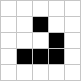
\includegraphics[scale=0.75]{Pictures/Glider}
	\caption{\label{Glider}Conway's Game of Life "Glider"}
\end{figure}

\subsection{\label{Convolution} Convolution}

A 2D convolution is a function that takes in a 2D matrix and a kernel. The kernel is usually smaller matrix that is "slid" over the larger matrix. Convolutions are largely used in neural networks and computer vision applications. 2D convolutions are especially useful in cellular automaton applications due to matrix math being much more optimized then for loops.

\begin{figure}[ht]
	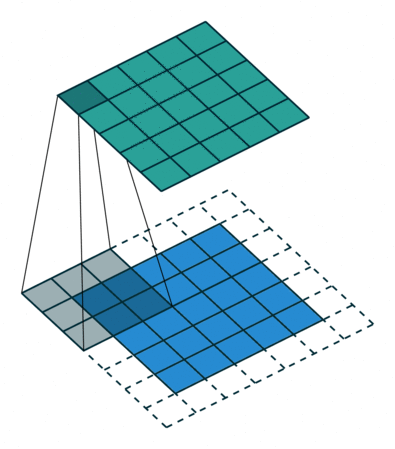
\includegraphics[scale=0.5]{Pictures/StaticConvolution}
	\caption{\label{2DConvolutionFig}2D convolution with zero padding and a 3x3 kernel}
\end{figure}

\section{\label{Method}Method}

The firefighting simulation is set as a set of 2D matrices. Each of the matrices represent a property of the simulation that include which tree's are on fire and the age of the tree's. On each simulation step, tree age's are incremented by the simulation step size. The amount of mass a tree has is proportional to the age of the tree. The mass increases until the tree is 100 years old, after which the tree mass rapidly decreases until it is 120 years old at which point the tree is dead.

The spreading of tree's from an alive space to a dead space uses a 2D convolution. The 2D convolution is between the the mass matrix to a 3x3 matrix of value 0.01. This equates to 1\% chance for each fully grown tree around a dead space for the dead space to grow a new tree. For tree's which are not at full mass, the chance they give is linearly proportional to the current vs adult mass. This results in young or old tree's still having a chance to spread but not at the same rate. The tree mass matrix is then check for any negative values and sets these indexes to 0, equating to having a tree fully die.

At the end of each time step, a random floating point value between 0-1 is generated. If the value generated is below 5E-5, a random tree is set on fire. This equates to approximately 13 years between fire events. This allows the forest enough time to recover and equates to the small chance some embers from a lightning strike or human caused fires growing large enough to start a fire on the forest scale.

When their is a fire event going on, a binary matrix with the binary value for each tree being on fire is multiplied element by element by the normalized tree mass in each cell. A 2D convolution is then done with a 5x5 kernal with a Gaussian distribution (Fig. \ref{GuassDist}).
	
\begin{figure}[ht]
	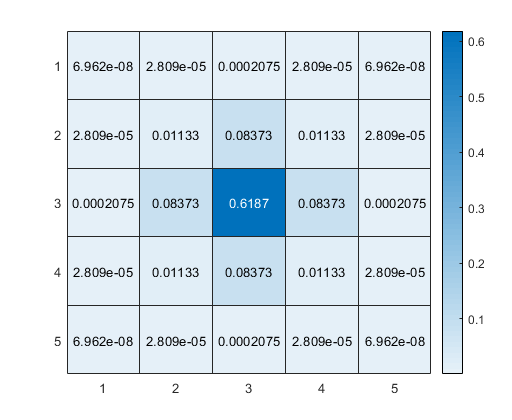
\includegraphics[scale=0.7]{Pictures/Guassian}
	\caption{\label{GuassDist} 5x5 Gaussian Kernel}
\end{figure}	

\section{\label{Results}Results}

\begin{figure}[ht]
	\includegraphics[scale=0.5]{Pictures/ForestImage}
	\caption{\label{SimulationSlice} Single frame of simulation. Lighter areas have more mass}
\end{figure}

Four different methods of fire fighting were tested. Over quenching in which 4 out of 5 fires are never even started which is equivalent to extremely proactive firefighting. No protection in which fires are not started or put out. Cutting down trees in a 3x3 area when a region of trees reaches a critical mass. Finally there was starting a fire in the center of a region when the mass of the region reached a critical mass and the region was not touching any of the edge cells of the matrix. Ten runs of the 4 different strategies were simulated over the course of 1000 years each. This totaled to over 60 GB of data to process and calculate.

By comparing the graphs for starting fires (Fig. \ref{StartFire}) to the graphs for no protection and cutting down trees (Fig. \ref{CutTrees},\ref{NoProtect}), the starting fire has a smaller density of higher mass burned and fraction of edges burned then the other strategies.

\begin{figure}[ht]
	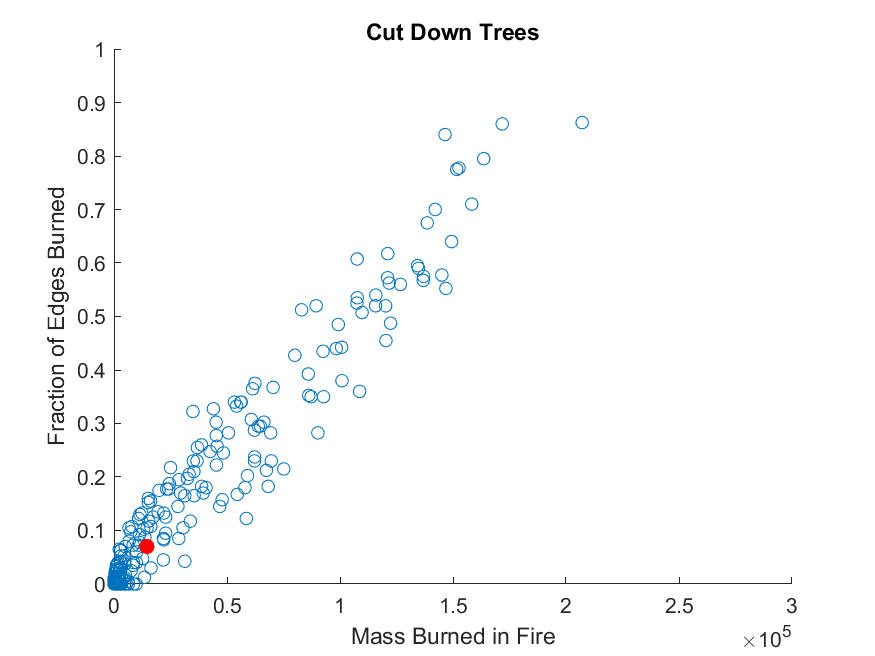
\includegraphics[scale=0.6]{Data/CutDownTrees}
	\caption{\label{CutTrees} Cutting Down Trees Data}
\end{figure}
\begin{figure}[ht]
	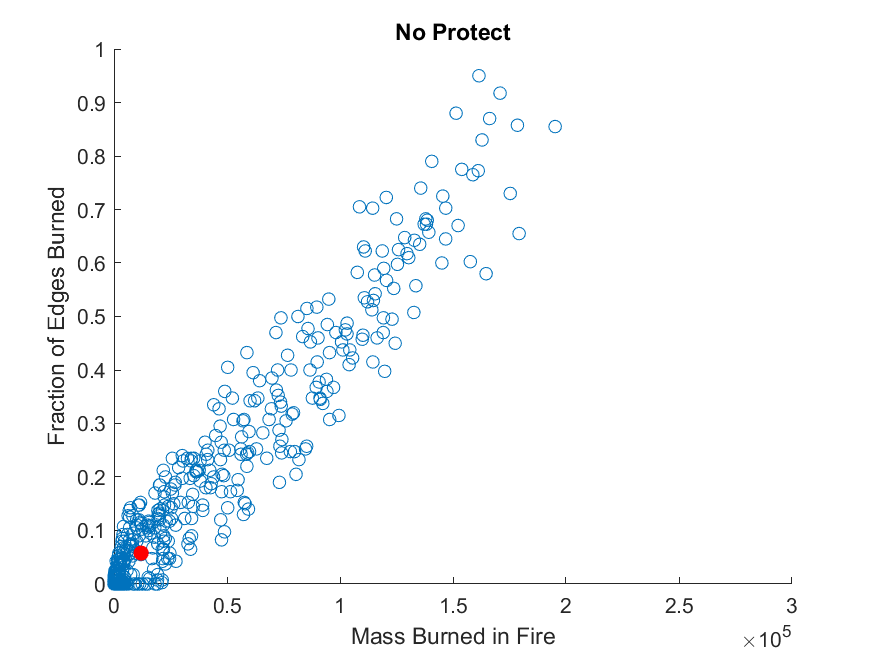
\includegraphics[scale=0.6]{Data/NoProtect}
	\caption{\label{NoProtect} Control Data}
\end{figure}
\begin{figure}[ht]
	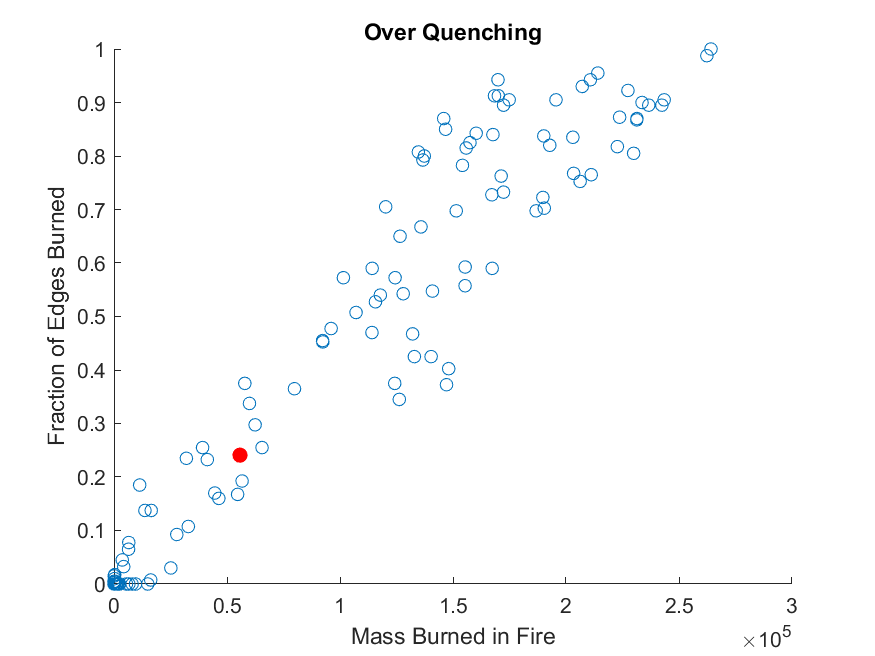
\includegraphics[scale=0.6]{Data/OverQuenching}
	\caption{\label{OverQuenching} Over Quenching Data}
\end{figure}
\begin{figure}[ht]
	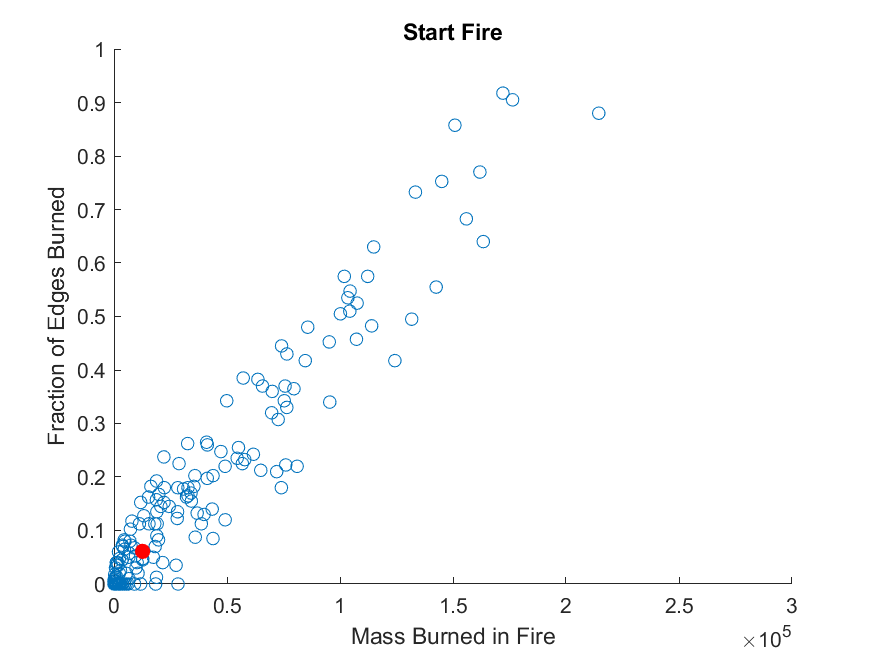
\includegraphics[scale=0.6]{Data/StartFire}
	\caption{\label{StartFire} Start Fire Data}
\end{figure}

\begin{table*}[b]%[H] add [H] placement to break table across pages
	\caption{\label{ProcessedData}Processed Data from Simulations}
	\begin{ruledtabular}
		\begin{tabular}{c||p{3cm}|p{3cm}|p{3cm}|p{3cm}}
			Strategy&
			Avg Mass (Tons) per Fire&
			Avg Fraction Edge Burned per Fire&
			Avg Acres Burned per Fire&
			Total Acres Burned per 1000 years\\
			\colrule
			Cut Down Trees & $0.512$ & $1.952$ & $1.952$ & $1.952$\\
			No Protection & $0.512$ & $1.952$ & $1.952$ & $1.952$\\
			Over Quenching & $0.512$ & $1.952$ & $1.952$ & $1.952$\\
			Starting Fire’s & $0.512$ & $1.952$ & $1.952$ & $1.952$\\
		\end{tabular}
	\end{ruledtabular}
\end{table*}


\section{\label{FutureWork}Future Work}

Improvements include implementing climate simulation such as dry seasons or years decreasing the rate of tree growth and increasing their flammability. With this improvement, different regions can be simulated from the rainy Midwest to the hot and dry west.

Future work could also include implementing wind biasing on fire spreading such that a strong wind to the west would decrease the chance a fire would spread to the east but increase the chance to spread to the west.

\begin{figure}[ht]
	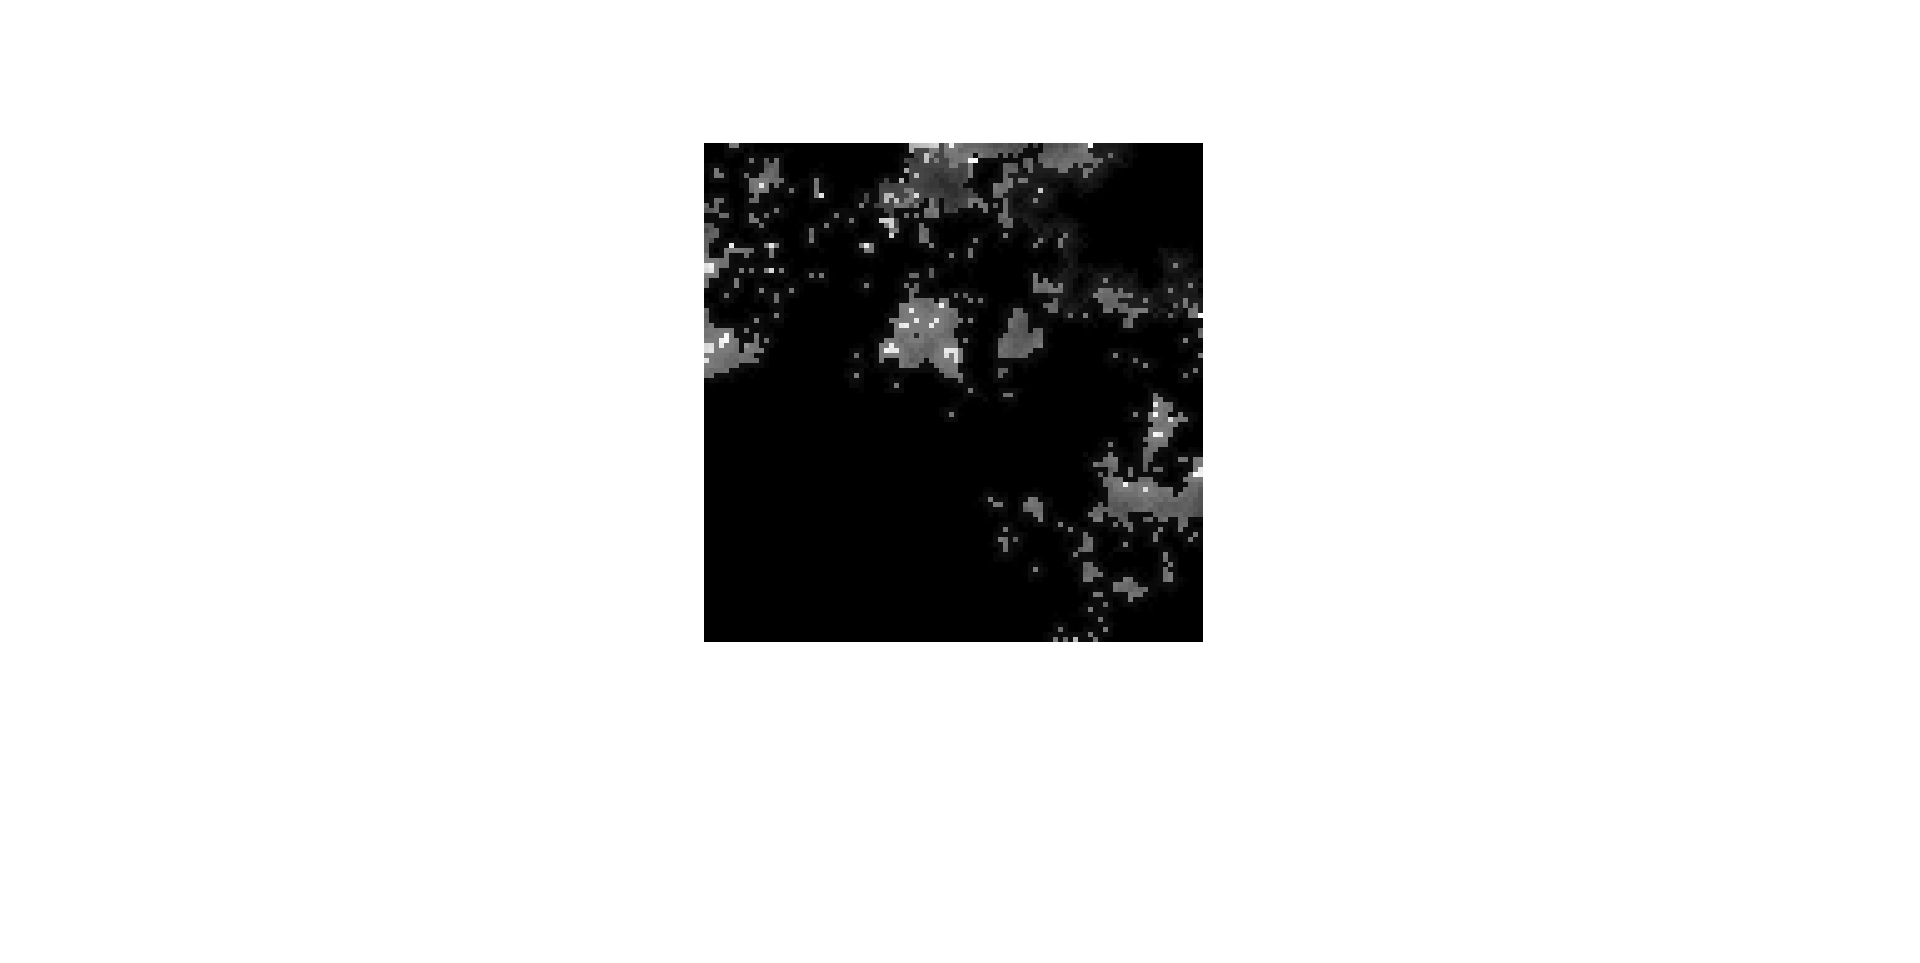
\includegraphics[scale=0.5]{Pictures/Threshold/Original}
	\caption{\label{ThreshOrig} Original slice of data}
\end{figure}
\begin{figure}[ht]
	\includegraphics[scale=0.5]{Pictures/Threshold/Threshold20}
	\caption{\label{Thresh20} Thresholding 20\% of max mass}
\end{figure}
\begin{figure}[ht]
	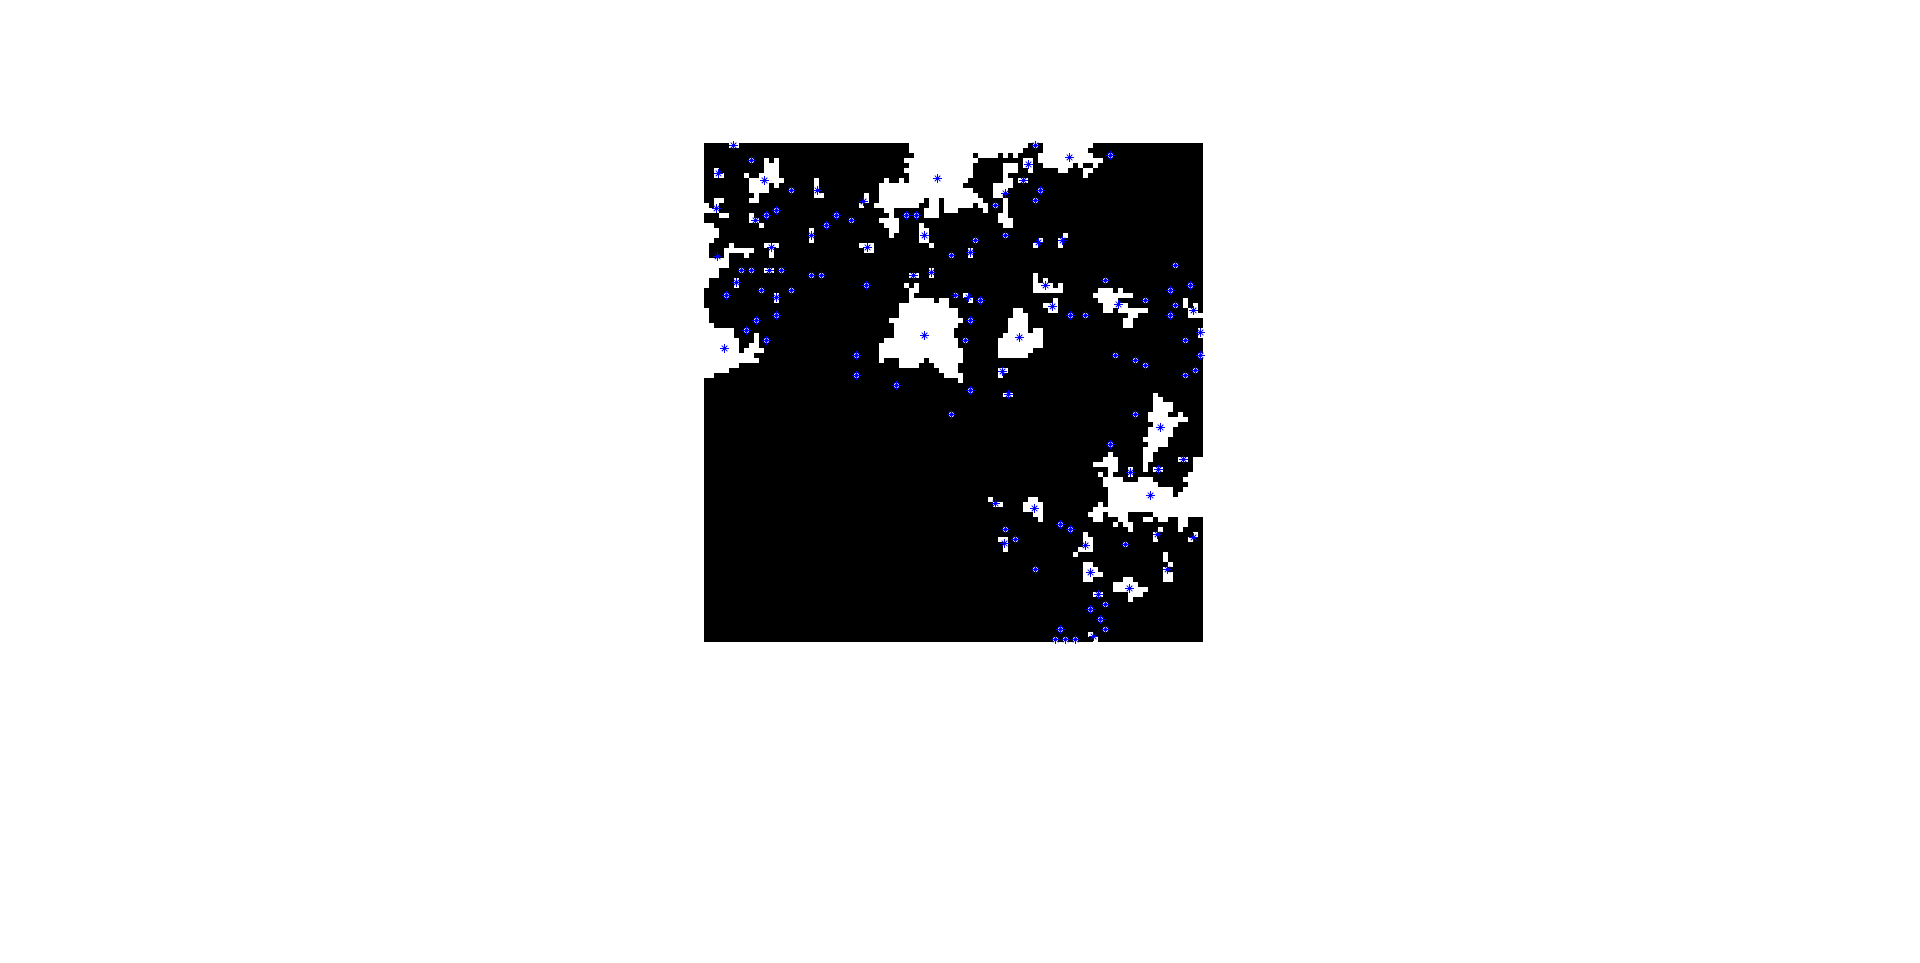
\includegraphics[scale=0.5]{Pictures/Threshold/Centroid}
	\caption{\label{Centroid} Centroid of thresholded region}
\end{figure}

%\subsection{}
%\subsubsection{}

% If in two-column mode, this environment will change to single-column
% format so that long equations can be displayed. Use
% sparingly.
%\begin{widetext}
% put long equation here
%\end{widetext}

% figures should be put into the text as floats.
% Use the graphics or graphicx packages (distributed with LaTeX2e)
% and the \includegraphics macro defined in those packages.
% See the LaTeX Graphics Companion by Michel Goosens, Sebastian Rahtz,
% and Frank Mittelbach for instance.
%
% Here is an example of the general form of a figure:
% Fill in the caption in the braces of the \caption{} command. Put the label
% that you will use with \ref{} command in the braces of the \label{} command.
% Use the figure* environment if the figure should span across the
% entire page. There is no need to do explicit centering.

% \begin{figure}
% \includegraphics{}%
% \caption{\label{}}
% \end{figure}

% Surround figure environment with turnpage environment for landscape
% figure
% \begin{turnpage}
% \begin{figure}
% \includegraphics{}%
% \caption{\label{}}
% \end{figure}
% \end{turnpage}

% tables should appear as floats within the text
%
% Here is an example of the general form of a table:
% Fill in the caption in the braces of the \caption{} command. Put the label
% that you will use with \ref{} command in the braces of the \label{} command.
% Insert the column specifiers (l, r, c, d, etc.) in the empty braces of the
% \begin{tabular}{} command.
% The ruledtabular enviroment adds doubled rules to table and sets a
% reasonable default table settings.
% Use the table* environment to get a full-width table in two-column
% Add \usepackage{longtable} and the longtable (or longtable*}
% environment for nicely formatted long tables. Or use the the [H]
% placement option to break a long table (with less control than 
% in longtable).
% \begin{table}%[H] add [H] placement to break table across pages
% \caption{\label{}}
% \begin{ruledtabular}
% \begin{tabular}{}
% Lines of table here ending with \\
% \end{tabular}
% \end{ruledtabular}
% \end{table}

% Surround table environment with turnpage environment for landscape
% table
% \begin{turnpage}
% \begin{table}
% \caption{\label{}}
% \begin{ruledtabular}
% \begin{tabular}{}
% \end{tabular}
% \end{ruledtabular}
% \end{table}
% \end{turnpage}

% Specify following sections are appendices. Use \appendix* if there
% only one appendix.

%\appendix*
%\section{\label{PythonMeanSigmaCalc}Python program to calculate mean and standard deviation}


% If you have acknowledgments, this puts in the proper section head.
%\begin{acknowledgments}
% put your acknowledgments here.
%\end{acknowledgments}

% Create the reference section using BibTeX:
\bibliography{FireBib}

\end{document}